\documentclass[USenglish,oneside,twocolumn]{article}

\usepackage[utf8]{inputenc}%(only for the pdftex engine)
%\RequirePackage[no-math]{fontspec}%(only for the luatex or the xetex engine)
\usepackage[big]{dgruyter_NEW}
\usepackage{subcaption}
\usepackage{afterpage}
%\DOI{foobar}

%\cclogo{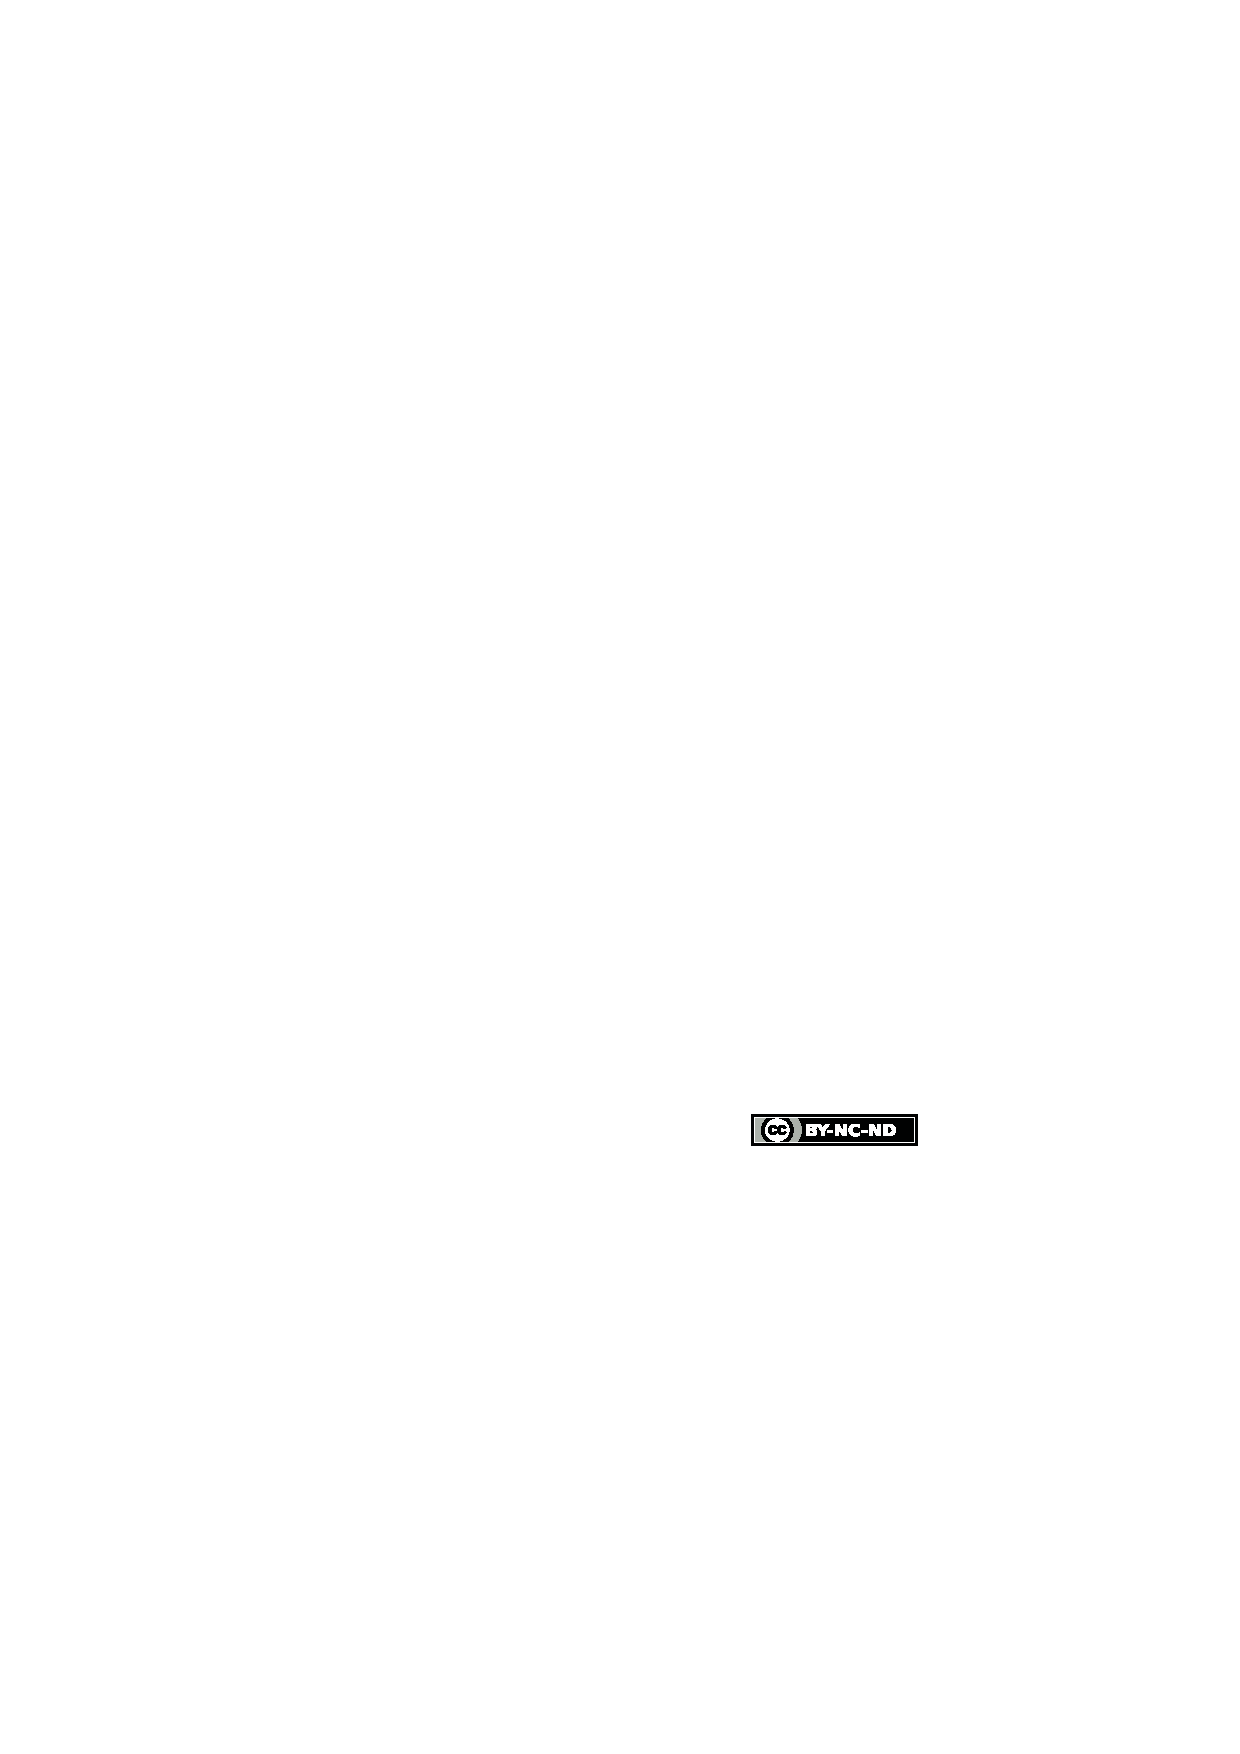
\includegraphics{by-nc-nd.pdf}}
  
\begin{document}
 
\author[1]{Bin Wang, Virat Shejwalkar}

\title{\Large Assignment 2: Performance Analysis of TCP Variants}

\runningtitle{Computer Networks}

\journalname{Computer Networks Fall}
  
 

\maketitle
\section{Introduction}
With growing network sizes, congestion issue becomes more and more pressing. Early TCP implementations considered only the buffer size of receiving node overlooking congestion possibilities. Increased network sizes introduced congestion issue which incrementally gave rise to various TCP variants. It is important to understand their key properties that help avoid congestion and study interplay of these variants so that it can be extrapolated to actual networks. In this regard, we perform three experiments with broad motivations to study performance variation of standalone TCP variants under variable loads, performance and fairness of combinations of TCP variants subject to a Constant Bit Rate (CBR) source (to imitate real world with various operating system employing spectrum of TCP variants) and effect of different queuing mechanisms on TCP variants when under constant network load. The TCP variants used are Tahoe, Reno, New Reno, Vegas and Sack. To model congestion, CBR source is used and it's flow rate is varied as required.

In experiment 1, we found that compared to other TCP variants evaluated (Tahoe/Reno/NewReno), Vegas not only display a more consistent throughput performance under different traffic conditions, but also has the least round trip time and package drop rate on average. However, under certain conditions the advantage of Vegas will become smaller or even disappear.

In experiment 2, we observed that bandwidth capacity occupied by different TCP varients are usually not euqal when they share the same bottleneck link. For example, in the NewReno/Reno experiment we found that NewReno will occupy more bandwidth than Reno as congestion level increases. In the NewReno/Vegas experiment, we found that NewReno outperform Vegas in almost all cases, and in the worst case scenario the bandwidth occupied by Newreno is more than five times as much as the bandwidth occupied by Vegas. This is mainly due to the different congestion control policy employed by TCP variants: some variants will increase their congestion window more aggressively than others and thus occupy more bandwidth.

From experiment-3 we found that under constant CBR rate, DropTail throughput is more than RED throughput due to the corresponding packet queuing/dropping mechanisms which indeed is because RED is more fair to other flows on a link than DropTail. We experiment to see best fit for RED from Reno/Sack under high/low congestion conditions; we found that under high congestion RED-Sack would work the best otherwise under low congestion, DropTail-Reno/Sack would perform equally

\section{Methodology}
For all the three experiments, we use the network simulator tool: ns-2 and to generate results and plots we use python scripts.\\
\noindent \textbf{Experiment-1}
Latency, throughput and packet drop are the representatives of performance of TCP variants and hence we use them throughout the experiments. In addition to the bandwidth occupied by the CBR flow which is varied in range \(1-10\) Mb, we are also varying the following parameters to represent different real-world scenarios:
\begin{itemize}
	\item The size of CBR packets. Although we used wireshark to see that the common size of UDP packet is 1000 bytes, we also tested other packet sizs to see its effect. We used CBR packets of 100, 200, 500, and 1000 bytes for our experiments.
	\item The start time of the CBR flow. In our experiments we do not the TCP run time (for 20 seconds in simulation time). Instead we are changing the starting\_time(CBR) - starting\_time(TCP) ranging in \{-1, 0.1, 1, 5, 10\} seconds. And once the CBR flow starts, it will continue until five seconds after the TCP flow stops.
	\item The latency of each link. We use three values for the latency of each link: 1ms, 10ms, and 100ms. With these values we are trying to represent three real-world scenarios: intra-datacenter networking, inter-AS networking, and inter-continental networking.
\end{itemize}
From the trace files, we calculate throughput over time, average throughput, average round trip time, and average packet drop rate. The main question we address here is if there exists an overall \textit{best} TCP variant and under what circumstances do it perform well. \\
\noindent \textbf{Experiment-2}
The main goal here is to see how TCP variants treat each other in congested environments. To identify fairness among TCP variants, the average throughput for each flow is the most appropriate measure. We also measured other metrics including round trip time, packet drop rate, data received by corresponding sink nodes in successive 1-second intervals from start of the flow, cumulative throughput over time. We think that fairness among TCP variants should also be reflected in recovery of TCP flows when CBR is started.\\
\noindent \textbf{Experiment-3}
Here, instead of CBR we try to vary queuing disciplines viz. DropTail and Random Early Drop(RED). The experiment is conducted for two TCP variants viz. Reno and Sack. In the experiment, we keep link capacity, latency and queue size same and equal to - 10Mb, 10ms and 10 respectively. We try to address the effects of the two queuing mechanisms on throughput, bandwidth consumption, latency (and RTT) and packet-drop rate on the aforementioned TCP variants. For bandwidth consumption, we extrapolate the results of throughput over time and of data received in successive time windows of 1 second; the reason for this is explained in the results. We measure the time difference between the time of queuing of packet at N1 and the time of reception of the packet at N4 as E-to-E latency of each packet. For RTT calculation, we measure the difference between the time of queuing of packet at N1 and the time of reception of \textit{ack} with same sequence number. The experiment is run for 10 seconds to capture different phases of TCP. To see if any particular combination of the considered TCP variants and queuing mechanism work better, we calculate parameters representing average packet-drop rate, throughput, RTT and latency.
\section{Experimental Results and Discussion}
\subsection{Experiment-1}
\begin{figure*}
	\centering
	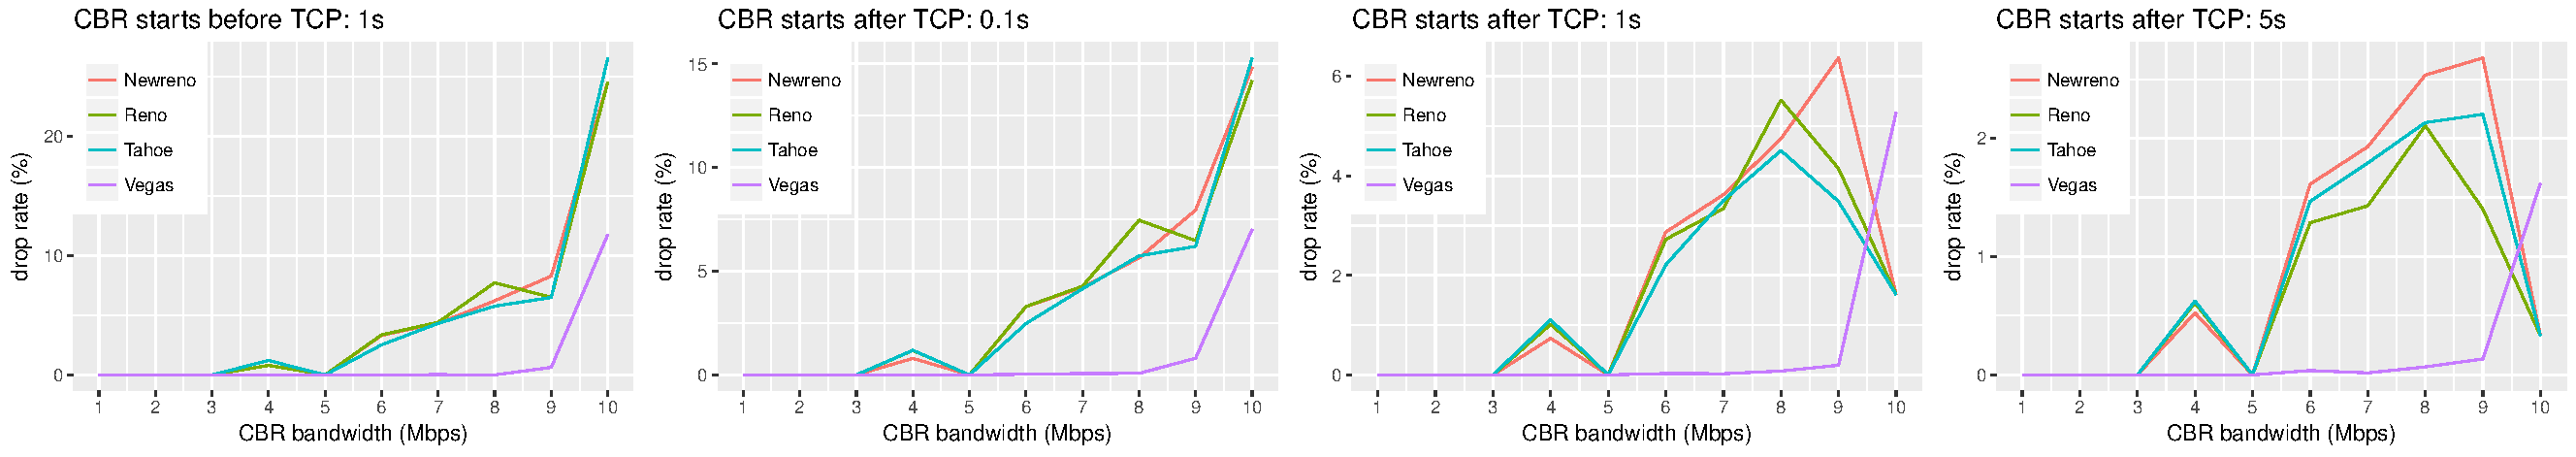
\includegraphics[width=\linewidth]{fig/experiment1/drop_rate.pdf}
	\captionsetup{justification=centering}
	\caption{Drop rate over CBR bandwidth with different CBR start time}
	\label{drop rate over bandwidth with start time}
	
	
	
	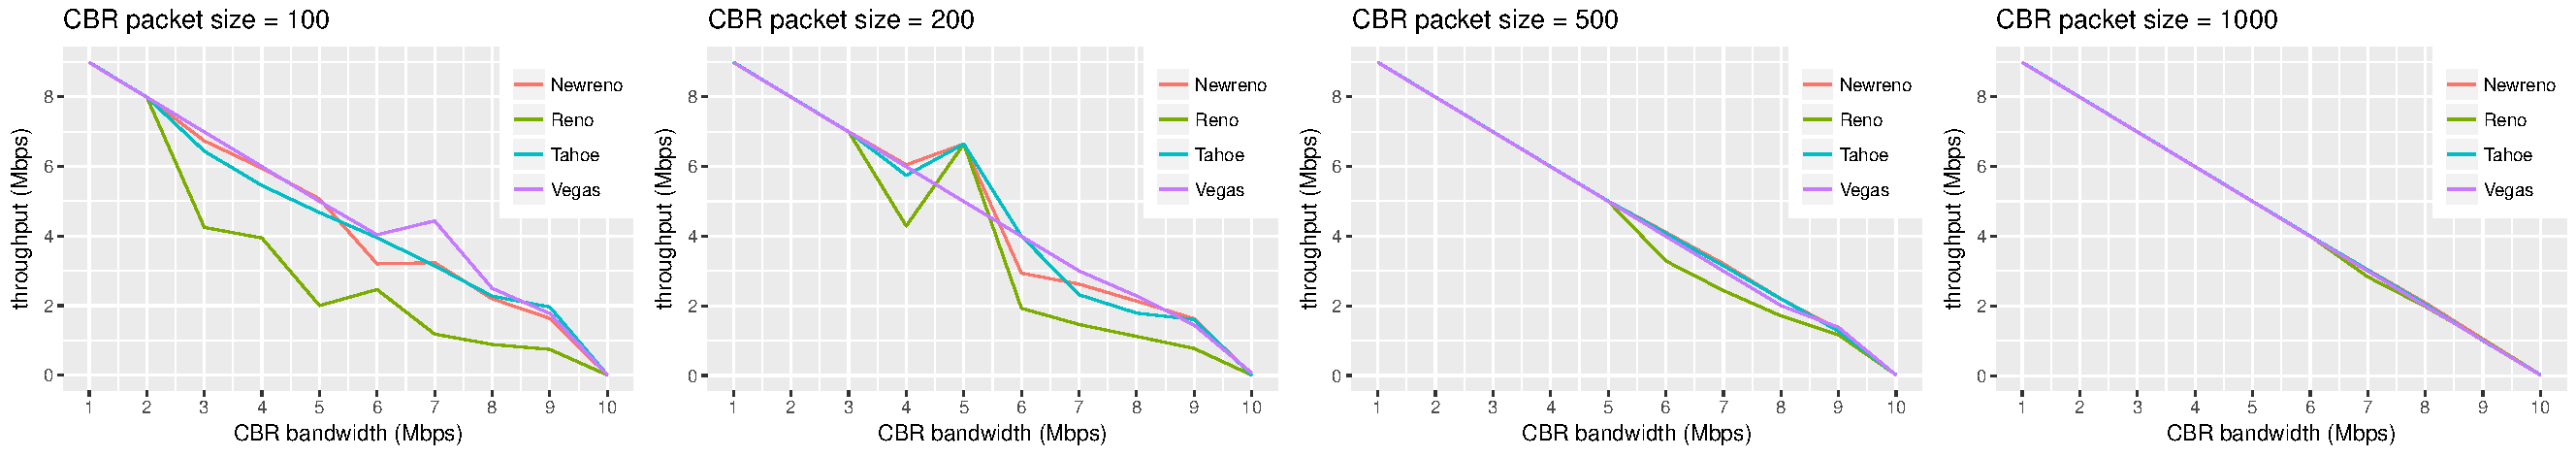
\includegraphics[width=\linewidth]{fig/experiment1/throughput.pdf}
	\captionsetup{justification=centering}
	\caption{Throughput over CBR bandwidth with different CBR packet size}
	\label{throughput over bandwidth with packet size}
\end{figure*}

\noindent \textbf{Drop rate:}
As shown in Fig. \ref{drop rate over bandwidth with start time}, Vegas ont only has the least average drop rate but is also more stable: it barely drops packets unless the bandwidth occupied by flow CBR is higher than 8Mbps. We also compared the drop rate of TCP variants with the CBR flow starting at different time. Note that in the third graph (where CBR flow starts 1 second after TCP starts) and the fourth graph (where CBR flow start 5 seconds after TCP starts) it seems that Vegas has a higher drop rate than the other three variant when the CBR bandwidth is at 10 Mbps. We traced these experiments and found that the actual reason is that Tahoe/Reno/Newreno almost stop sending packets quickly after the CBR flow starts (the congestion window dropped to near zero), while Vegas was is able to send data at a certain rate. Therefore, we think Vegas better than other alternatives in terms of drop rate.

\noindent \textbf{Throughput:} In general, the TCP throughput dcreases as the bandwidth capacity occupied by the CBR flow increases. However, the change patterns of throughput displayed by different are somewhat different: as shown in Fig. \ref{throughput over bandwidth with packet size} that the thoughput of Reno changes radically in a wide range as the congestion level increases, while the throughput of Vegas chages more smoothly. 

We also found that in addition to CBR bandwidth, other parameters will also affect TCP behavior dramitically, such as the CBR packet size. For the CBR flow we have \(bandwidth = packet\_size \times send\_rate\). Therefore , when CBR bandwidth is fixed, the smaller the CBR packets are, the more CBR packets there will be on the fly in the network at any given time. Obvously, TCP will have a higher drop rate with smaller CBR packets since the average queue length for each link will beacome larger. However, as shown in Fig. \ref{throughput over bandwidth with packet size}, the throughput of TCP variants changes more smmothly as the CBR packet size becomes larger and all TCP variants behaves almost the same when the CBR packet size is 1000 bytes. 

\noindent \textbf{Latency:} We measured the round trip time with different latency per link: 1ms, 10ms, and 100ms. Experiment results show that Vegas has a much lower round trip time than other TCP variants in high-speed networks. However, as the link latency increases the advantage of Vegas becomes smaller. When link latency is 100ms, all TCP variants seem to have the same round trip time.

\noindent \textbf{Conclusion:} To sum up, we think Vegas is the "best" TCP variant for all the three metrics that we evaluated. But under certain circumstances its advantage may become smaller or even unnoticable.


\subsection{Experiment-2}

The term TCP fairness refers to that if a bottleneck link is shared by multiple TCP connections, the bandwidth used by each connection should be equal. Therefore, the only metric we will consider in this experiment is bandwidth. Fig. \ref{throughput fairness} shows the bandwidths of two TCP sharing a bottleneck link over the CBR bandwidth. It can be seen that when the two TCP connections are the same variant the fairness between connections basically holds. However, if two connections are different variants, the difference between their bandwidths are noticable: for the NewReno/Reno experiment, when the CBR bandwidth is larger than 3Mbps, the throughput of NewReno is better than Reno; for the NewReno/Vegas experiment, NewReno outperforms Vegas in all tests. In worst case the throughput of NewReno is more than five times as much as the throughput of Vegas.

To validate the statistical significane, we set CBR bandwidth to 5Mbps and run the experiment 100 times for each set of TCP matchup. However, in NS2 when parameters are fixed every run of the simulation will yield exactly the same result, thus making running the same experiment multiple times meaning less. To work around this problem, we vary the start time of the CBR flow for each run: for each run we start the CBR flow randomly from 1s to 2s before we start the TCP flows. In theory, as long as the CBR flow starts before the TCP flow, the difference in start time doesn't matter since the CBR flow sends packet at a constant rate. But in reality, starting CBR flow at random times will make the network state at the moment that TCP flows start slightly different, thus yielding different experiment result. Therefore, CBR start time is the only parameter we can vary to introduce randomness for each run.

We calulated the ratio of \(throughput_{N1-N4}\) to \(throughput_{N5-N6}\) for each run, and then calculated the statistics for each set of experiments. The statistics are shown in Tab. \ref{Throughput statistics}. The unfair phenomenon between NewReno and Vegas are very obious: the difference between ratio(NewReno/Vegas) and ratio(Vegas/Vegas) is huge and each run gives almost the same result. However, for the comparison between Reno and NewReno the result is not that obvious: as shown in Fig. \ref{ratio histogram} even when the two TCP connection sharing the bottleneck link are both Reno, experiments show that flow from N1 to N4 will usually perform better than flow from N5 to N6. Therefore, we need to eliminate the possibility that NewReno outperforming Reno is due to some random reason. We use R to perform T-test on the two samples from NewReno/Reno experiment and Reno/Reno experiment, the calculated t-value is \(-13.825\) and the p-value is less than \(2.2e-16\). This means that we can basically falsify the alternative hypothesis that the difference between NewReno/Reno and Reno/Reno is equal to zero since its possibility is close to zero.

\noindent \textbf{Explanation:} In the NewReno/Reno experiment, when CBR bandwidth there is no unfairness between NewReno and Reno. This is because in this situation there are nearly no dropped packets therefore NewReno and Reno are both mainly in the slow start and congestion avoidance periods. In these two periods NewReno and Reno have exactly the same behavior so they have the same throughput. However, as CBR bandwidth increases there are more and more packet drops. In this case NewReno will have an advantage over Reno since NewReno can handle multiple packet drops: NewReno doesn't exit fast recovery until all the packets at the time when it entered fast recovery are acknowledged.

In the NewReno/Vegas experiment, we can see NewReno will always occupy more bandwidth than Vegas. This is because in the slow start period NewReno increases the congestion window more aggressively: the congestion window of NewReno is incremented exponentially while the congestion window of Vegas is incremented by 1 at a time. And as the network congested, Vegas will notice the congestion earlier since increase in round trip time happens before packets start to drop. Therefore, Vegas will reduce its congestion window earlier than NewReno, giving out even more bandwidth to NewReno.

These results are very interesting since in Experiment 1 we have shown that Vegas is the best TCP variant in our evalution. But in reality its performance will suffer severe downgrade since other more aggressive TCP variants such as NewReno will seize much more bandwidth. For that reason, Vegas has rarely been used in real-world other than in laboratory settings.

\begin{figure*}
	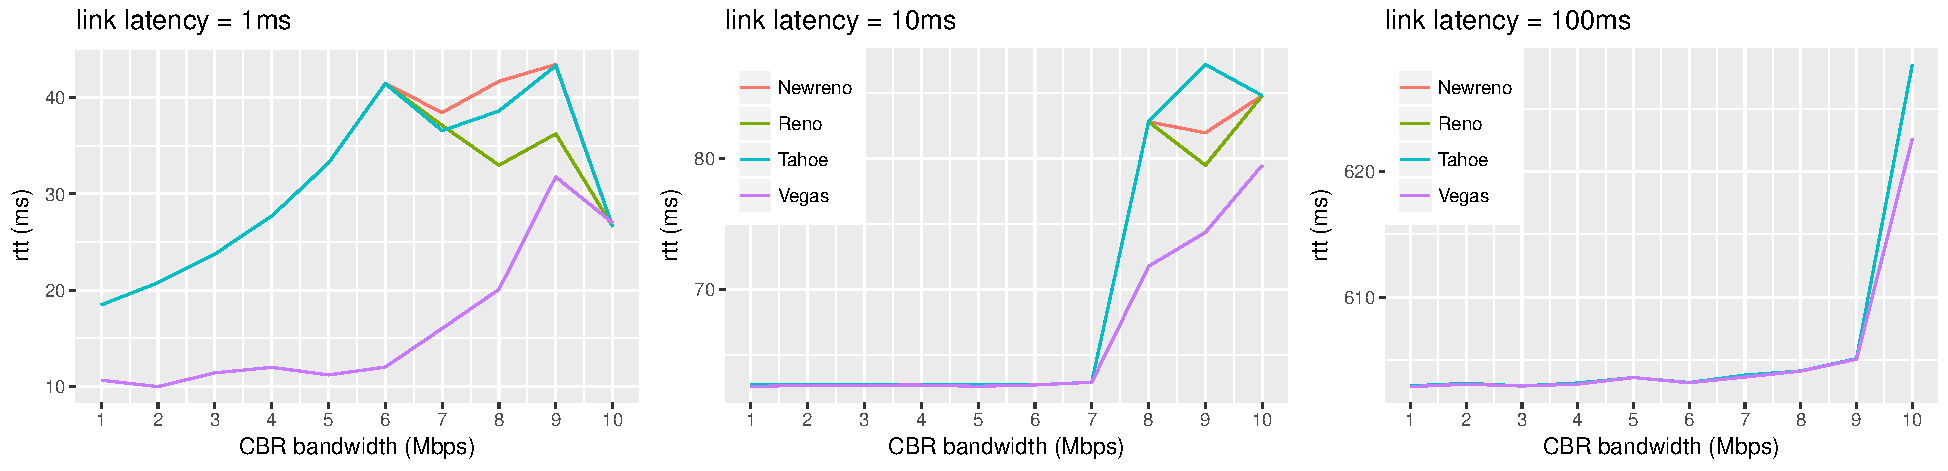
\includegraphics[width=\linewidth]{fig/experiment1/rtt.pdf}
	\captionsetup{justification=centering}
	\caption{Throughput over CBR bandwidth with different CBR packet size}
	
	
	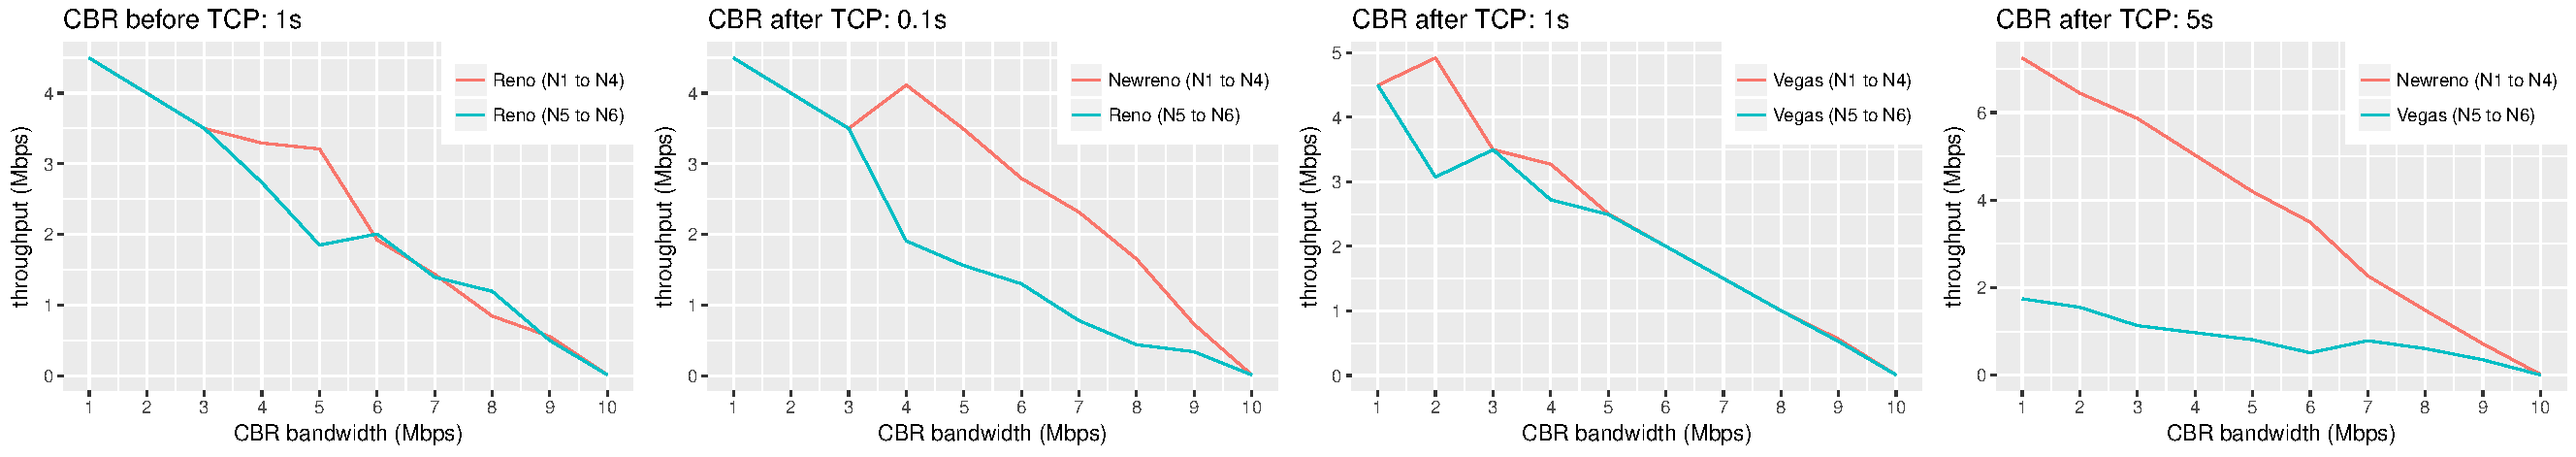
\includegraphics[width=\linewidth]{fig/experiment2/throughput.pdf}
	\captionsetup{justification=centering}
	\caption{Throughput comparison of two TCP variants sharing a bottleneck link}
	\label{throughput fairness}
\end{figure*}


\begin{table}
	\begin{tabular}{| l | l | l | l | l | l |}
		N1 to N4 & N5 to N6 & Mean & Std dev & skewness & kurtosis \\ \hline
		Reno & Reno & 1.22 & 0.51 & -0.35 & -1.61 \\ \hline
		NewReno & Reno & 2.23 & 0.53 & 2.62 & 8.34 \\ \hline
		Vegas & Vegas & 1 & 0 & -0.91 & -1.18 \\ \hline
		NewReno & Vegas & 5.17 & 0 & -1.41 & 0.25 \\ 
	\end{tabular}
	\captionsetup{justification=centering}
	\caption{Statistics of \(\dfrac{Trhoughput_{N1-N4}}{Throughput_{N5-N6}}\) samples}
	\label{Throughput statistics}
\end{table}

\begin{figure}
	\centering
	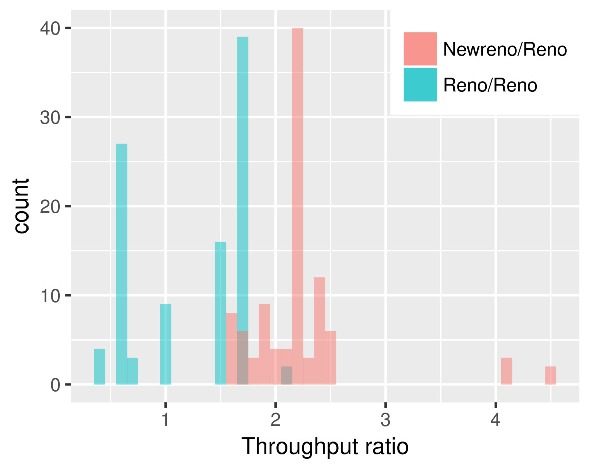
\includegraphics[width=\linewidth]{fig/experiment2/throughput_ratio.pdf}
	\captionsetup{justification=centering}
	\caption{Histogram of throughput ratio samples collected in Reno/Reno and NewReno/Reno experiments}
	\label{ratio histogram}
\end{figure}


\subsection{Experiment-3}
The main question that we try to address is - if there exists is a TCP variant/queuing mechanism combination that works better than the others and under what network settings. The exhaustive list of components that contribute to the performance of a TCP variant is - queuing mechanism, queue size, link capacity or available bandwidth, link latency, CBR flow-rate, difference in time of start of CBR. But not all are required to conclude the better policy. Calculating the bandwidth available for TCP when CBR is started is tricky to find, because as UDP is stateless, packet losses are invisible. Hence, we consider the ratio of available bandwidth for TCP and for CBR as the ratio of throughputs of the two flows as observed at the corresponding sink nodes. We also consider the data received at both CBR and TCP sink nodes in successive time intervals of 1 second. This can give us an estimate of the ratio of data of TCP and CBR available on a link in that time interval which can be used to estimate the available bandwidth for TCP.\\

\noindent\textbf{Bandwidth Fairness}: To see when TCP flow stabilizes \textit{for the first time}, we plot congestion window of the TCP flow for all the combinations. It can be seen from the Fig.\ref{cwind_dt} that, for DropTail, at around $t = $2 seconds the TCP flow becomes stable for both the TCP variants; similar behavior is observed for RED as well.
\begin{figure}[h]
\captionsetup{justification=centering}
    \centering
    \begin{subfigure}{0.5\linewidth}
        \centering
        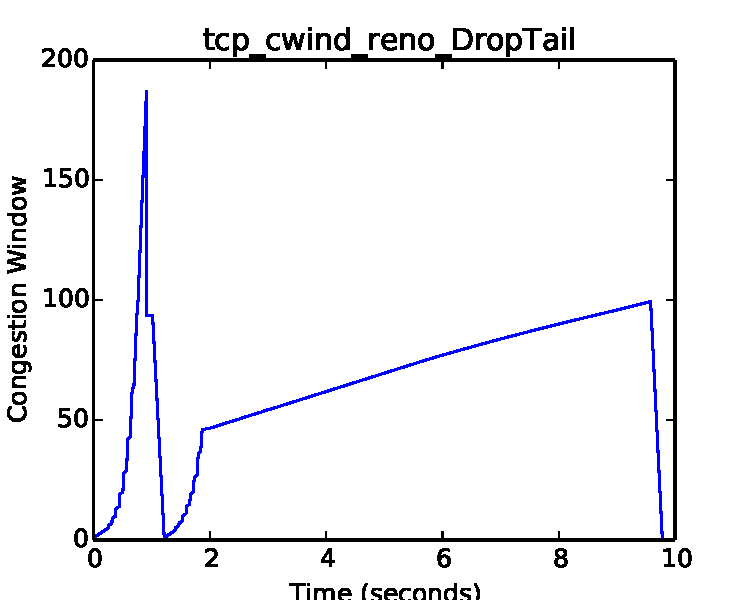
\includegraphics[width=\linewidth]{fig/tcp_cwind_reno_DropTail.pdf} % first figure itself
        %\caption{Reno}
    \end{subfigure}\hfill
    \begin{subfigure}{0.5\linewidth}
        \centering
        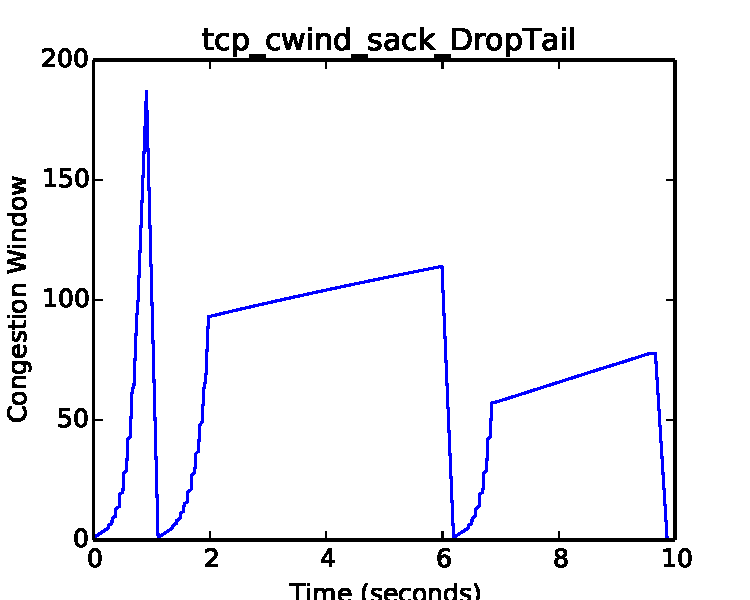
\includegraphics[width=\linewidth]{fig/tcp_cwind_sack_DropTail.pdf} % second figure itself
        %\caption{Sack}
    \end{subfigure}
\caption{Congestion Window for DropTail}
\label{cwind_dt}
\end{figure}

\begin{figure}
\captionsetup{justification=centering}
    \centering
    \begin{subfigure}{0.5\linewidth}
        \centering
        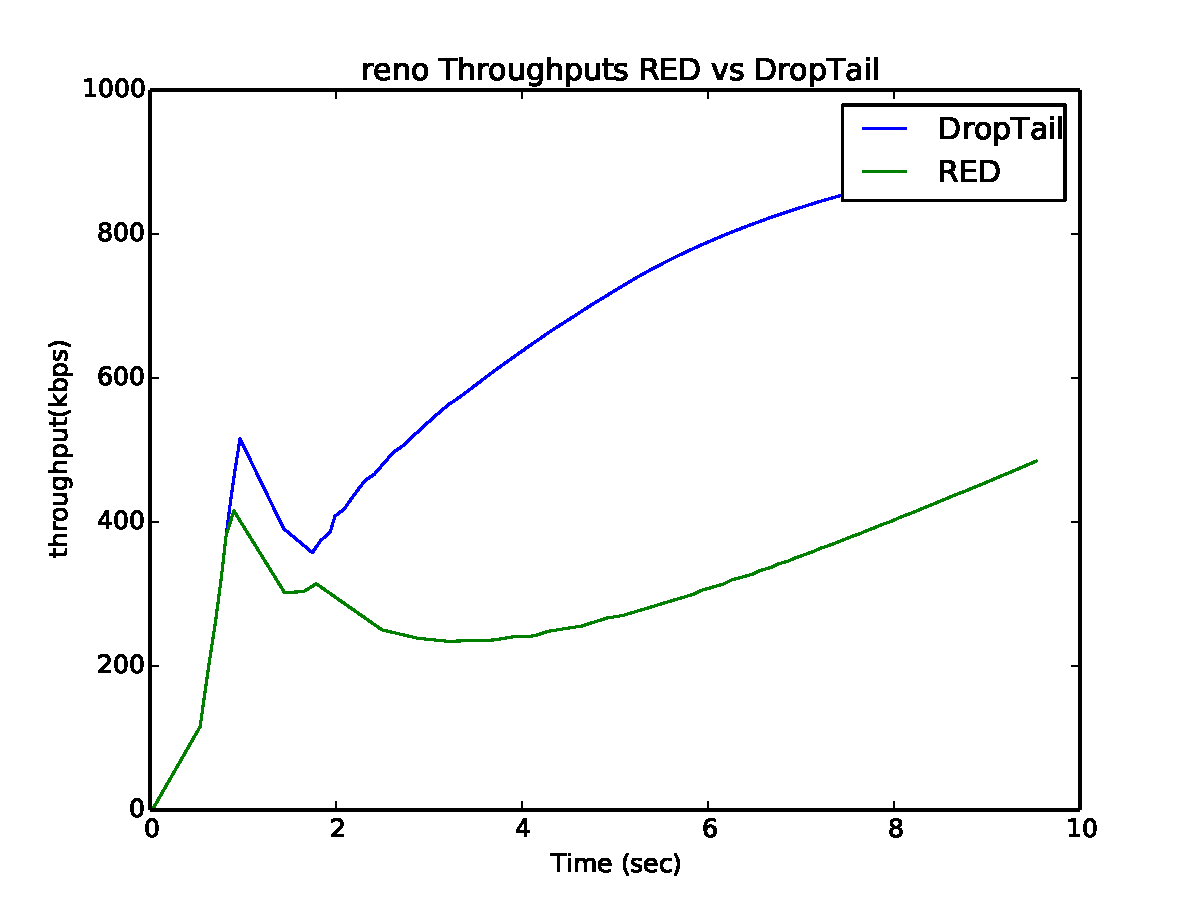
\includegraphics[width=\linewidth]{fig/Reno_throughput_RED_DT.pdf} % first figure itself
        %\caption{Reno}
    \end{subfigure}
    \begin{subfigure}{0.48\linewidth}
        \centering
        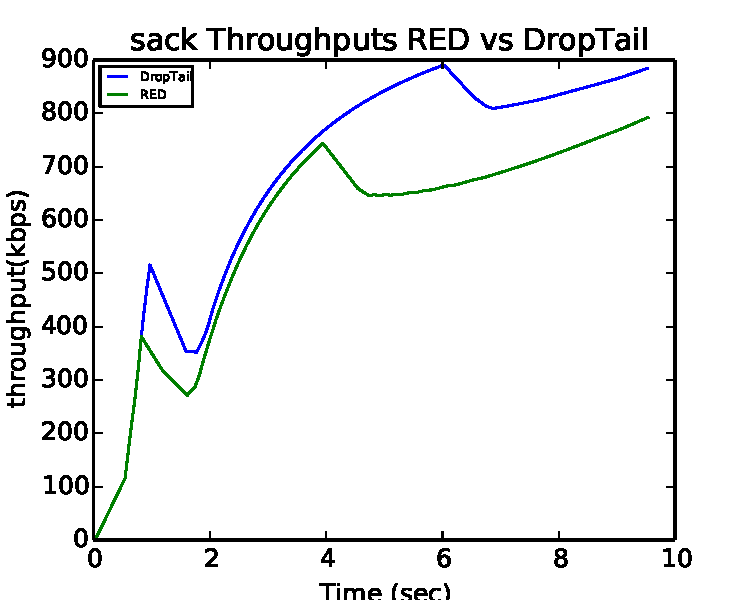
\includegraphics[width=\linewidth]{fig/Sack_throughput_RED_DT.pdf} % second figure itself
        %\caption{Sack}
    \end{subfigure}
\caption{Throughput - RED vs DropTail}
\label{red_vs_dt}
\end{figure}

Fig.\ref{red_vs_dt} shows the output for each TCP variant plotted to compare the effects on their cumulative throughput over time under the two queuing mechanisms. Cumulative throughput $TP$ at time $t'$ here is $$TP(t') = {\sum_{t \in (0,t')}p(t) \over t'}$$ where $p(t)$ is size of packer received at time $t$. It is clear from the plots that in both the cases of Reno and Sack DropTail provides better cumulative throughput over time. We also calculated the average throughput, which can be seen from the cumulative throughput plots as the last throughput value. In case of average throughput as well, the DropTail mechanism seems to excel over RED. The reason for the DropTail dominance is the basic way in which the two queuing mechanisms differ. As RED drops packets with a probability which is based on the number of packets in queue at any time, it is very likely that in spite of free space, an incoming packet will be dropped. However, DropTail start dropping incoming packets only when the queue is full. The plots also support this hypothesis. 

As mentioned before, to compare the available bandwidths for a TCP variant over queuing mechanisms, we calculate throughputs in each time intervals and see the difference when queuing mechanisms are switched. From Fig.\ref{intervals}, dominance of DropTail over RED is visible. In case of Sack TCP, RED performs 
\begin{figure}[h]
\captionsetup{justification=centering}
    \centering
    \begin{subfigure}{0.5\linewidth}
        \centering
        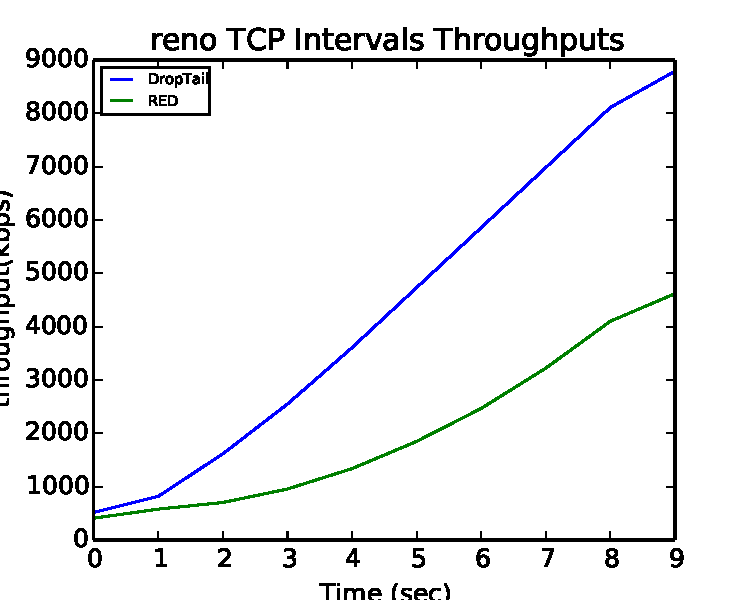
\includegraphics[width=\linewidth]{fig/reno_intervals_RED_DT.pdf} % first figure itself
        %\caption{Reno}
    \end{subfigure}
    \begin{subfigure}{0.48\linewidth}
        \centering
        \includegraphics[width=\linewidth]{fig/Sack_intervals_RED_DT.pdf} % second figure itself
        %\caption{Sack}
    \end{subfigure}
\caption{Throughput Over Interval}
\label{intervals}
\end{figure}

Fig.\ref{bw_sack} and Fig.\ref{bw_reno} show how the two queuing mechanisms treat CBR and TCP flows in terms of throughput over time when CBR rate is kept constant at 3mb. Note that we extrapolate this results to conclude available bandwidth for each flow under the corresponding queuing mechanisms. It can be seen from Fig.\ref{red_vs_dt}, Fig.\ref{bw_sack} and Fig.\ref{bw_reno} that in case of TCP Reno, DropTail performs way better than RED while for TCP Sack, DropTail slightly outperforms RED. Hence, RED is fairer than DropTail to the other flows as with RED, TCP does not consume all the bandwidth that it can but looks for congestion and if it's high gives other flow chance to send it's packets.\\
\begin{figure}[h]
\captionsetup{justification=centering}
    \centering
    \begin{subfigure}{0.5\linewidth}
        \centering
        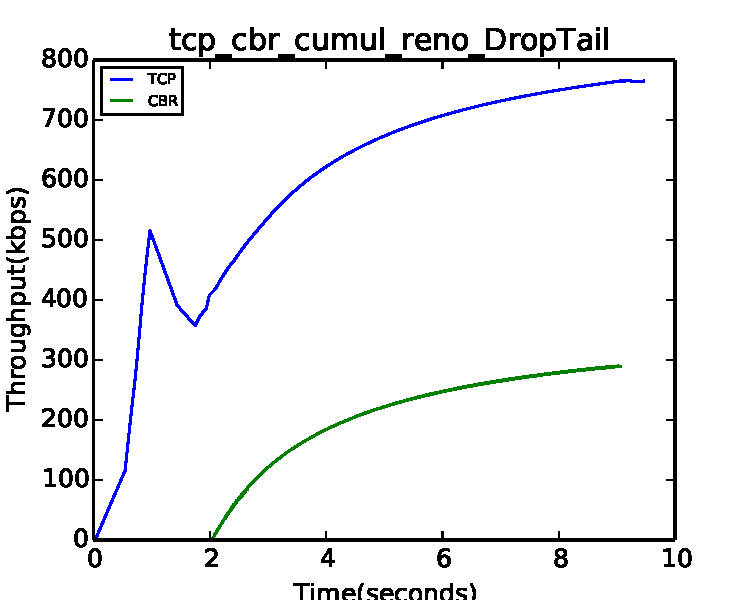
\includegraphics[width=\linewidth]{fig/tcp_cbr_cumul_3mb_reno_DropTail.pdf} % first figure itself
        %\caption{DropTail}
    \end{subfigure}
    \begin{subfigure}{0.48\linewidth}
        \centering
        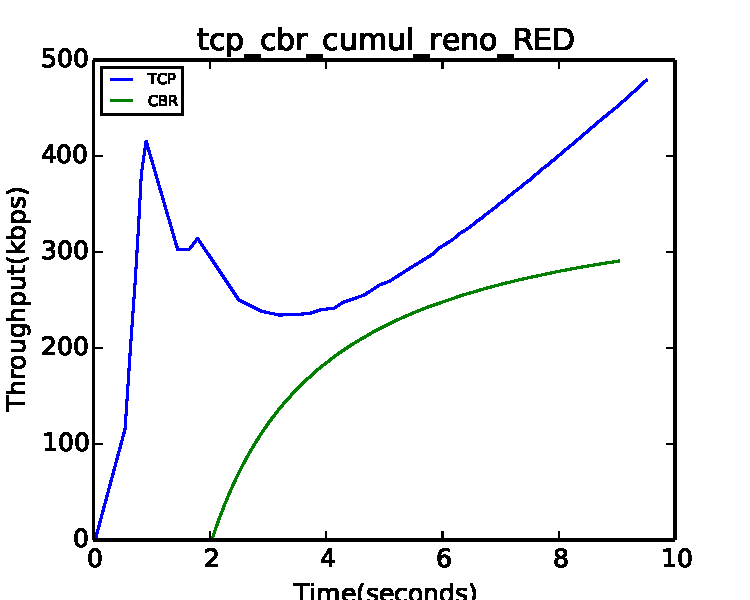
\includegraphics[width=\linewidth]{fig/tcp_cbr_cumul_3mb_reno_RED.pdf} % second figure itself
        %\caption{RED}
    \end{subfigure}
\caption{Throughput TCP Reno vs CBR}
\label{bw_reno}
\end{figure}

\begin{figure}
\captionsetup{justification=centering}
    \centering
    \begin{subfigure}{0.5\linewidth}
        \centering
        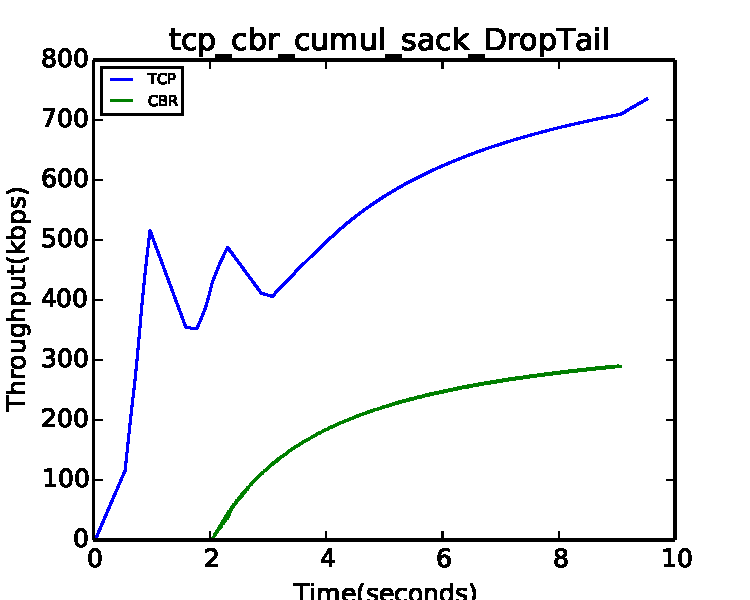
\includegraphics[width=\linewidth]{fig/tcp_cbr_cumul_3mb_sack_DropTail.pdf} % first figure itself
        %\caption{DropTail}
    \end{subfigure}
    \begin{subfigure}{0.48\linewidth}
        \centering
        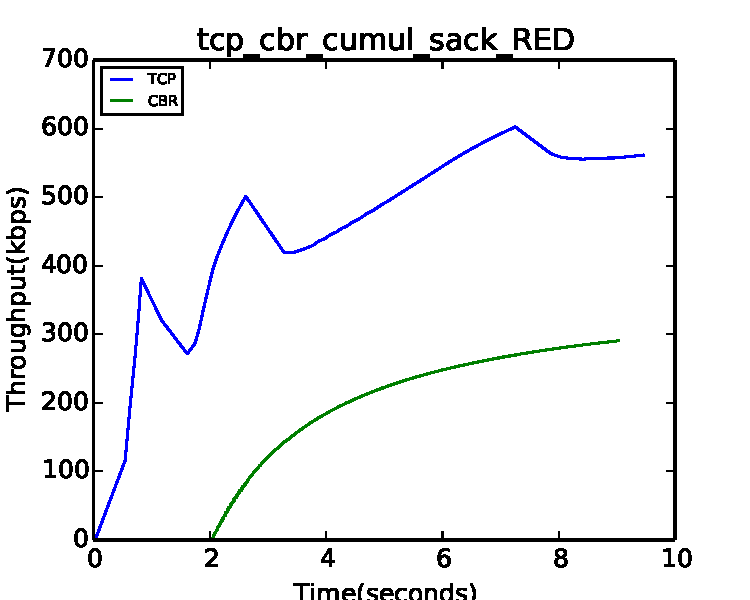
\includegraphics[width=\linewidth]{fig/tcp_cbr_cumul_3mb_sack_RED.pdf} % second figure itself
        %\caption{RED}
    \end{subfigure}
\caption{Throughput TCP Sack vs CBR}
\label{bw_sack}
\end{figure}

\noindent \textbf{Latency of TCP Packets}: We calculated end-to-end latency and round trip time for all the TCP packets that are received at N4 with CBR rate 3mb. We use delayed acknowledgments\cite{DelAck} for this experiment. From the plots Fig.\ref{latency} and average latency values (sack-DropTail:0.0486, sack-RED:0.036, reno-DropTail:0.0507, reno-RED:0.0343) it can be seen that the latency is more for DropTail that for RED. This is expected because, RED with it's probabilistic queuing/dropping of packets handles congestion better than DropTail which queues packets just based on available space. This difference in congestion handling is more effectively seen in RTT calculations.\\
\begin{figure}
\captionsetup{justification=centering}
    \centering
    \begin{subfigure}{0.5\linewidth}
        \centering
        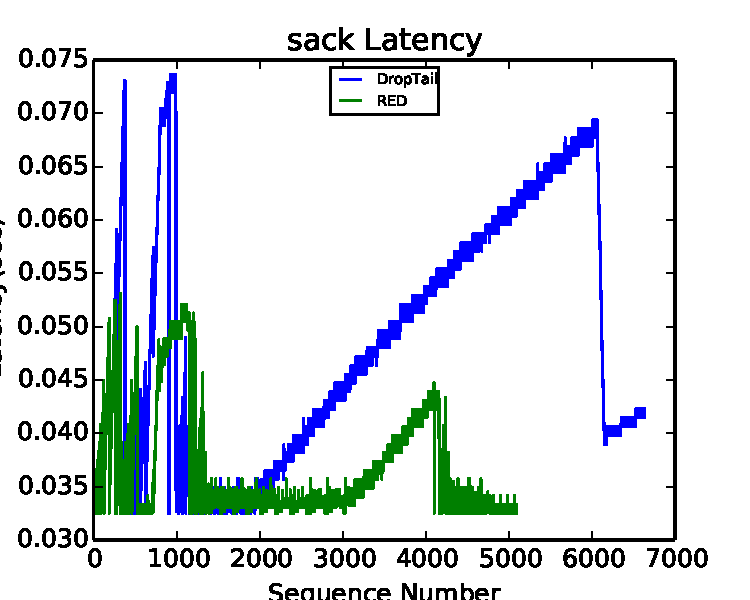
\includegraphics[width=\linewidth]{fig/sack_latency.pdf} % first figure itself
        %\caption{DropTail}
    \end{subfigure}
    \begin{subfigure}{0.48\linewidth}
        \centering
        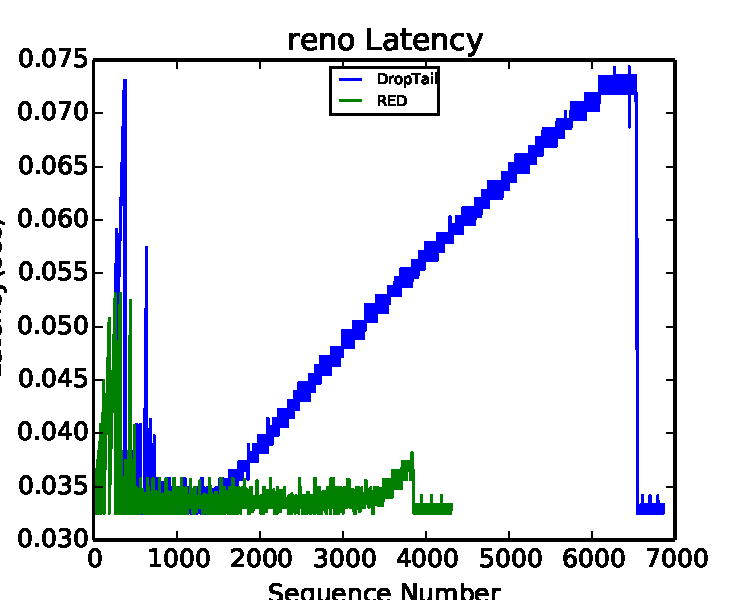
\includegraphics[width=\linewidth]{fig/reno_latency.pdf} % second figure itself
        %\caption{RED}
    \end{subfigure}
\caption{End-to-End Latency DropTail vs RED}
\label{latency}
\end{figure}

% \begin{figure}
% \captionsetup{justification=centering}
%     \centering
%     \begin{subfigure}{0.5\linewidth}
%         \centering
%         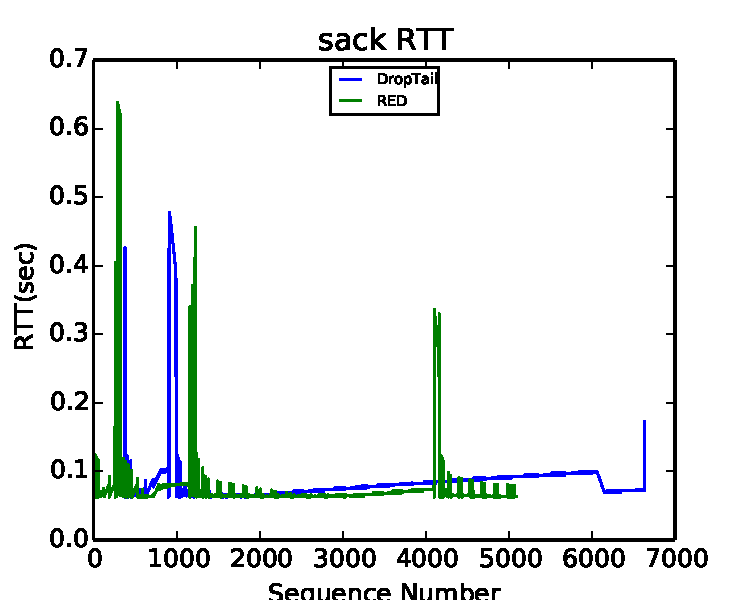
\includegraphics[width=\linewidth]{fig/sack_rtt.pdf} % first figure itself
%         %\caption{DropTail}
%     \end{subfigure}
%     \begin{subfigure}{0.48\linewidth}
%         \centering
%         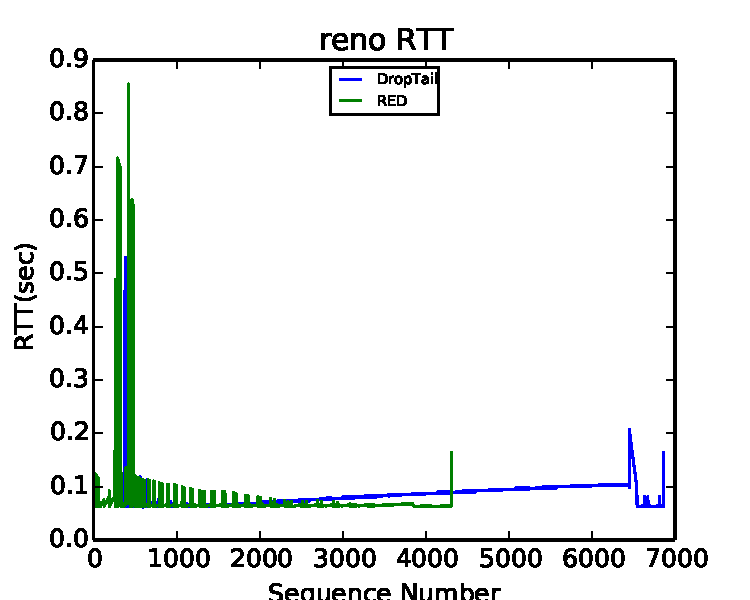
\includegraphics[width=\linewidth]{fig/reno_rtt.pdf} % second figure itself
%         %\caption{RED}
%     \end{subfigure}
% \caption{RTT DropTail vs RED}
% \label{rtt}
% \end{figure}
\noindent \textbf{Reaction of TCP to CBR start:} We start CBR, when TCP stabilizes for the first time. From Fig.\ref{bw_reno} and Fig.\ref{bw_sack}, we observe that in all the combinations, TCP throughput falls when CBR start; however, the difference is seen in recoveries. For TCP Reno, recovery with DropTail highly outperforms that with RED; for Sack the difference is not that notable. The similar recovery of Sack for RED and DropTail stems from low packet drop rates. Sack performs better if packet drop is high, and the higher packet drop rate in case of RED is the exact environment in which Sack performs well. This compensation causes low performance difference between DropTail and RED for Sack. This can also be seen in Fig.\ref{red_vs_dt} where Sack performance is similar for RED and DropTail.\\

\noindent \textbf{RED-Sack combination}: Direct consequence of the above reasoning is that is RED is the queuing mechanism used, packet drop rate will be higher than otherwise. Hence, it is important to use TCP variant which especially performs well with higher packet drop rate. Sack handles the situation perfectly hence, RED and Sack combination will be better than RED and Reno combination. To answer our main question of perfect combination, we think that RED being fairer than DropTail, on a link with multiple TCP flows RED would collectively perform better than DropTail. Hence, as RED - Sack go well hand-in-hand, in congestion-prone networks, RED-Sack should be chosen for better \textit{collective performance}. However, for not so congestion-prone networks, DropTail-Reno/Sack would perform equally as the performance difference in Reno and Sack is visible mainly with high packet drops.
%###################################################################



\begin{thebibliography}{99}
\bibitem{vincent} V.~Bindschaedler, R.~Shokri, Synthesizing Plausible Privacy-Preserving Location Traces, IEEE Symposium on Security and Privacy (S\&P) (2016)
\bibitem{DelAck} T.~Henderson, Delayed-ACK TCP Sink, https://www.isi.edu/nsnam/ns/doc/node407.html
\end{thebibliography}

\end{document}
